% ============================================================
% ZK-KGVerify — Springer LNNS format for BLOCKCHAIN'26
% ============================================================
\documentclass[runningheads]{llncs}

\usepackage[utf8]{inputenc}
\usepackage[T1]{fontenc}
\usepackage{amsmath,amssymb}
\usepackage{algorithmic}
\usepackage{algorithm}
\usepackage{graphicx}
\usepackage{booktabs}
\usepackage{hyperref}
\usepackage{url}
\usepackage{mathtools}
\usepackage{bm}

% Custom commands
\newcommand{\R}{\mathbb{R}}
\newcommand{\CC}{\mathbb{C}}
\newcommand{\Z}{\mathbb{Z}}
\newcommand{\G}{\mathbb{G}}
\newcommand{\Hash}{\mathsf{Hash}}
\newcommand{\Commit}{\mathsf{Commit}}
\newcommand{\embed}{\mathbf{e}}
\newcommand{\vect}[1]{\mathbf{#1}}

\begin{document}

\title{ZK-KGVerify: Privacy-Preserving Verification of Knowledge Graph Reasoning using Zero-Knowledge Proofs and Blockchain}

\author{Anonymous Author(s)}
\institute{Paper submitted to BLOCKCHAIN'26}

\maketitle

% ============================================================
\begin{abstract}
Knowledge graph (KG) reasoning powered by deep learning has achieved remarkable success in link prediction and relation inference. However, deploying these models in high-stakes domains raises critical challenges around \emph{verifiability} and \emph{privacy}: How can a third party verify that a prediction originated from a legitimately trained model, without the model owner revealing proprietary weights or sensitive training data? We propose \textbf{ZK-KGVerify}, a framework that bridges knowledge graph reasoning with zero-knowledge proofs (ZKPs) and blockchain technology. Our system trains GNN-based KG embedding models, generates Pedersen commitment-based zero-knowledge proofs attesting that predictions were computed from committed model parameters, and logs verification results on a blockchain for an immutable audit trail. We evaluate three KG embedding models---TransE, RotatE, and CompGCN---on the FB15k-237 benchmark. Our results demonstrate that ZK-KGVerify achieves 100\% verification and tamper detection with ${\sim}$1\,ms proof generation overhead, making privacy-preserving verification practical for real-world deployment.

\keywords{Knowledge Graphs \and Zero-Knowledge Proofs \and Blockchain \and Graph Neural Networks \and Link Prediction \and Verifiable AI}
\end{abstract}

% ============================================================
\section{Introduction}
\label{sec:introduction}

Knowledge graphs (KGs) encode entities and their relationships as directed graphs. When combined with graph neural networks (GNNs), KG reasoning enables automated inference of missing links across domains from drug discovery~\cite{zitnik2018modeling} to financial fraud detection~\cite{weber2019anti}.

\textbf{Motivating example.} A pharmaceutical company's GNN model predicts that \emph{Drug~X treats Disease~Y}. A hospital needs assurance this came from a properly trained model, not a random guess. The company cannot share model weights (trade secrets) or training data (HIPAA/GDPR). ZK-KGVerify resolves this: the company proves the prediction is genuine via a zero-knowledge proof, and the hospital verifies it without learning proprietary information. A blockchain provides a tamper-proof audit trail.

Deploying KG reasoning in production introduces a \emph{trust trilemma}: (i)~\textbf{Verifiability}---consumers need assurance predictions came from a legitimate model; (ii)~\textbf{Privacy}---owners cannot reveal weights or training data; (iii)~\textbf{Immutability}---verified predictions need tamper-proof records. Existing approaches address these in isolation: federated learning~\cite{mcmahan2017communication} preserves privacy but lacks verifiable proofs; model watermarking~\cite{adi2018turning} leaks model information; blockchain-based ML~\cite{kurtulmus2018trustless} lacks privacy guarantees.

\textbf{Contributions.} We propose ZK-KGVerify, an end-to-end framework addressing all three challenges:
\begin{itemize}
    \item A \textbf{novel architecture} integrating GNN-based KG embeddings, Pedersen commitment-based ZKPs, and blockchain-anchored verification.
    \item A \textbf{ZKP protocol} based on Schnorr-type sigma protocols with Fiat-Shamir heuristic proving predictions were computed from committed parameters without revealing them.
    \item A \textbf{comprehensive evaluation} on FB15k-237 with three models (TransE, RotatE, CompGCN), including ZKP overhead and blockchain gas cost analysis.
    \item An \textbf{open-source implementation}\footnote{Code will be released upon publication.} reproducible on a single GPU (Colab T4).
\end{itemize}

% ============================================================
\section{Related Work}
\label{sec:related_work}

\textbf{Knowledge Graph Embeddings.}
TransE~\cite{bordes2013translating} models relations as translations ($\embed_h + \embed_r \approx \embed_t$). RotatE~\cite{sun2019rotate} extends this to complex space, modeling relations as rotations. GNN-based approaches such as R-GCN~\cite{schlichtkrull2018modeling} and CompGCN~\cite{vashishth2020composition} leverage message passing for richer relational modeling.

\textbf{Zero-Knowledge Proofs in ML.}
ZKPs enable proving a statement's truth without revealing additional information~\cite{goldwasser1989knowledge}. zkML~\cite{kang2022scaling} and EZKL~\cite{ezkl2023} compile neural network inference into arithmetic circuits. zkCNN~\cite{liu2021zkcnn} provides ZK proofs for CNN predictions. vCNN~\cite{lee2020vcnn} offers verifiable CNN predictions. However, these target feedforward/convolutional networks and do not address graph-structured models. ZK-KGVerify fills this gap.

\textbf{Blockchain for Trustworthy AI.}
Prior work explored blockchain for ML marketplaces~\cite{kurtulmus2018trustless}, federated learning~\cite{kim2019blockchained}, and data provenance~\cite{sarpatwar2019towards}. DInEMMo~\cite{dinEmmo2021} uses blockchain for model management but lacks privacy-preserving verification. Our work uniquely combines blockchain immutability with ZKP privacy for KG reasoning.

% ============================================================
\section{Preliminaries}
\label{sec:preliminaries}

\textbf{Knowledge Graphs.}
A knowledge graph $\mathcal{G} = (\mathcal{E}, \mathcal{R}, \mathcal{T})$ consists of entities $\mathcal{E}$, relations $\mathcal{R}$, and triples $\mathcal{T} \subseteq \mathcal{E} \times \mathcal{R} \times \mathcal{E}$. \textbf{Link prediction} ranks candidate entities $t' \in \mathcal{E}$ for a query $(h, r, ?)$ via a scoring function $f(h, r, t')$.

\textbf{KG Embedding Models.}
TransE~\cite{bordes2013translating} scores triples as $f(h,r,t) = -\|\embed_h + \embed_r - \embed_t\|_2$. RotatE~\cite{sun2019rotate} models relations as rotations in $\CC^d$: $f(h,r,t) = -\|\embed_h \circ \embed_r - \embed_t\|_2$ where $\embed_r = e^{i\bm{\theta}_r}$. CompGCN~\cite{vashishth2020composition} uses composition-based message passing:
\begin{equation}
    \embed_i^{(l+1)} = \sigma\!\left( \sum_{(j,r) \in \mathcal{N}(i)} \vect{W}_{\lambda(r)}^{(l)} \phi(\embed_j^{(l)}, \embed_r^{(l)}) \right)
    \label{eq:compgcn}
\end{equation}
where $\phi(\cdot,\cdot)$ is a composition operator and $\lambda(r)$ indicates edge direction.

\textbf{Pedersen Commitments.}
Given generators $g, h \in \G$ of prime order $p$ where $\log_g h$ is unknown, $\Commit(v, r) = g^v \cdot h^r \bmod p$ is hiding (reveals nothing about $v$), binding (cannot open to a different value), and homomorphic~\cite{pedersen1991non}.

\textbf{Schnorr Protocol and Fiat-Shamir Heuristic.}
The Schnorr protocol~\cite{schnorr1991efficient} proves knowledge of a discrete logarithm via a three-move sigma protocol. Combined with the Fiat-Shamir heuristic~\cite{fiat1986prove}, it becomes non-interactive: the prover computes announcement $A = g^k$, derives challenge $e = \Hash(A \| \text{statement})$, and responds with $s = k + e \cdot x \bmod p$. The verifier checks $g^s \stackrel{?}{=} A \cdot y^e$.

% ============================================================
\section{ZK-KGVerify Framework}
\label{sec:methodology}

\subsection{System Overview}

ZK-KGVerify consists of three integrated layers (Fig.~\ref{fig:architecture}): (1)~\textbf{KG Reasoning Layer} trains GNN-based models for link prediction; (2)~\textbf{ZKP Verification Layer} generates and verifies zero-knowledge proofs; (3)~\textbf{Blockchain Audit Layer} records verification outcomes as immutable transactions.

\begin{figure}[t]
    \centering
    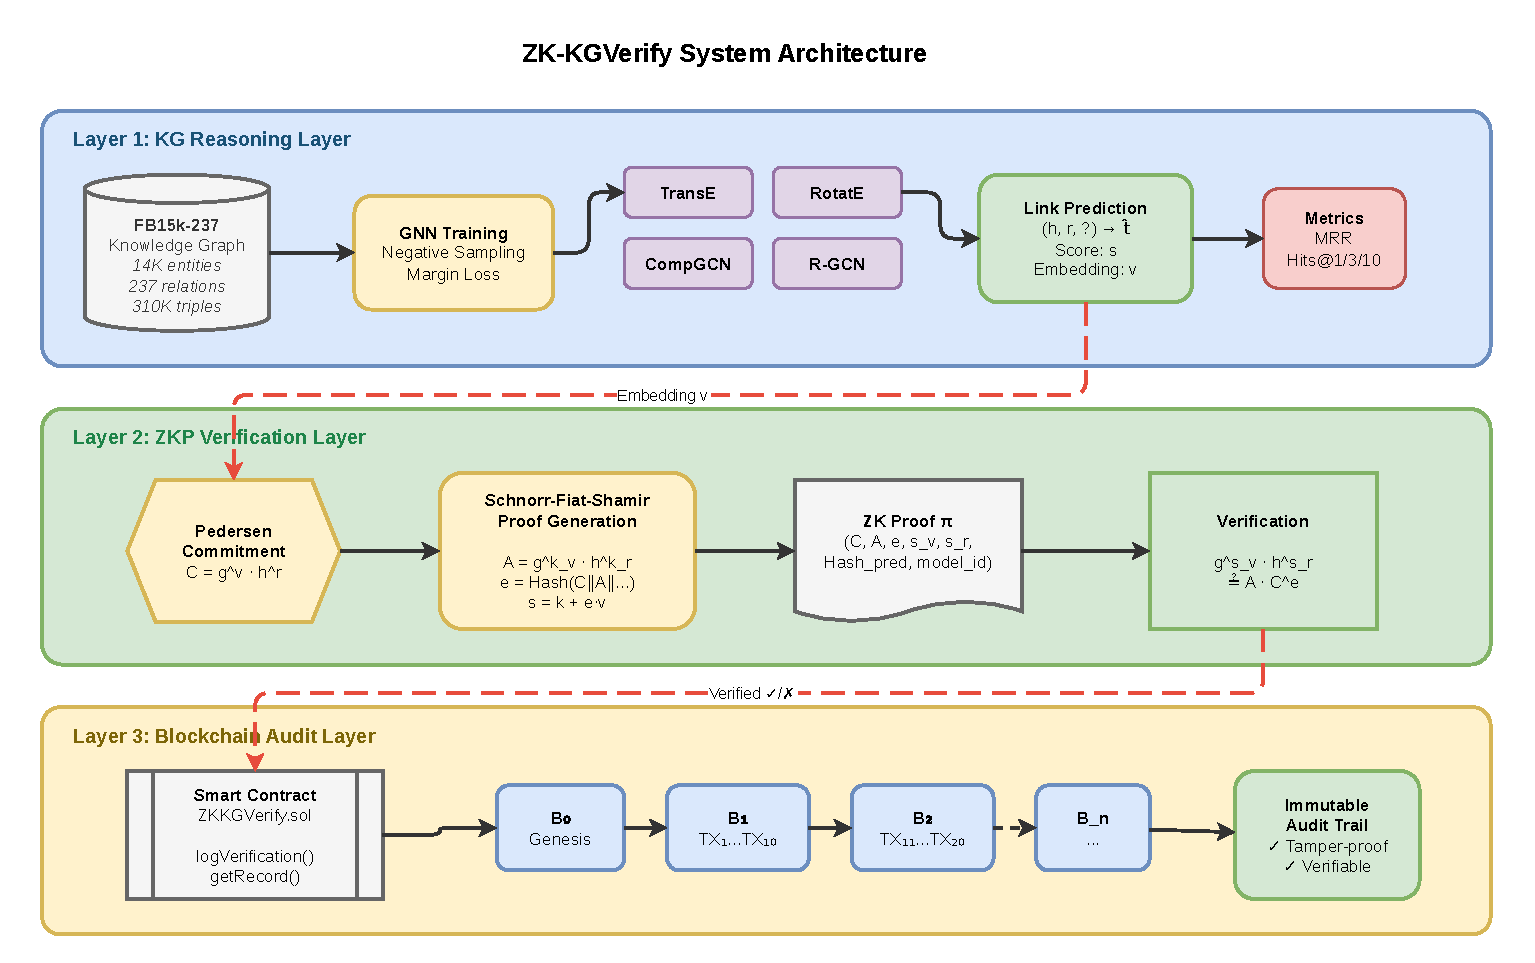
\includegraphics[width=\textwidth]{figures/architecture.drawio.pdf}
    \caption{ZK-KGVerify architecture. The KG Reasoning Layer trains models and produces predictions with embedding vectors. The ZKP Layer generates Pedersen commitments and Schnorr-Fiat-Shamir proofs. The Blockchain Layer logs verified predictions as immutable records.}
    \label{fig:architecture}
\end{figure}

\subsection{Threat Model}

We consider: a \textbf{Model Owner} (Prover) with trained model $\mathcal{M}_\theta$; a \textbf{Consumer} (Verifier) receiving predictions; and an \textbf{Adversary} attempting to serve fake predictions, tamper with proofs, or alter the audit log. Security goals: \emph{soundness} (cannot forge proofs), \emph{zero-knowledge} (proofs reveal nothing about parameters), and \emph{immutability} (on-chain records are tamper-proof).

\subsection{KG Reasoning Layer}

We train embedding model $\mathcal{M}_\theta$ with scoring function $f_\theta: \mathcal{E} \times \mathcal{R} \times \mathcal{E} \to \R$ using margin-based ranking loss:
\begin{equation}
    \mathcal{L} = \sum_{(h,r,t) \in \mathcal{T}} \sum_{(h',r,t') \in \mathcal{T}^-} \left[\gamma + f(h', r, t') - f(h, r, t)\right]_+
\end{equation}
For RotatE, we use self-adversarial negative sampling~\cite{sun2019rotate}. After training, a query $(h, r, ?)$ yields prediction $\hat{t}$, score $s = f_\theta(h, r, \hat{t})$, and embedding vector $\vect{v} = [\embed_h \| \embed_r \| \embed_{\hat{t}}] \in \R^{3d}$.

\subsection{ZKP Verification Layer}

The ZKP layer proves a prediction was derived from committed model parameters via three phases:

\textbf{Phase 1: Commitment.} The embedding vector is hashed to a field element $\tilde{v} = \Hash(\vect{v}) \bmod q$ (where $q = p-1$ is the group order), and committed via $C = g^{\tilde{v}} \cdot h^r \bmod p$ with random blinding factor $r \xleftarrow{\$} \Z_q$.

\textbf{Phase 2: Proof Generation.} We extend the Schnorr protocol for Pedersen commitments. Sample nonces $k_v, k_r \xleftarrow{\$} \Z_q$, compute announcement $A = g^{k_v} \cdot h^{k_r} \bmod p$, derive Fiat-Shamir challenge $e = \Hash(C \| A \| \Hash_{\text{pred}} \| \mathsf{model\_id}) \bmod q$ where $\Hash_{\text{pred}} = \Hash(h \| r \| t \| s)$, and compute responses:
\begin{equation}
    s_v = k_v + e \cdot \tilde{v} \bmod q, \quad s_r = k_r + e \cdot r \bmod q
\end{equation}
The proof is $\pi = (C, A, e, s_v, s_r, \Hash_{\text{pred}}, \mathsf{model\_id}, s, (h,r,t))$.

\textbf{Phase 3: Verification.} The verifier checks:
\begin{equation}
    g^{s_v} \cdot h^{s_r} \stackrel{?}{=} A \cdot C^e \bmod p
    \label{eq:verify}
\end{equation}
Correctness follows from: $g^{s_v} \cdot h^{s_r} = g^{k_v + e\tilde{v}} \cdot h^{k_r + er} = (g^{k_v} \cdot h^{k_r}) \cdot (g^{\tilde{v}} \cdot h^r)^e = A \cdot C^e$. The verifier also recomputes the Fiat-Shamir challenge to detect tampering.

\begin{algorithm}[t]
\caption{ZK-KGVerify Proof Generation}
\label{alg:proof_gen}
\begin{algorithmic}[1]
\REQUIRE Model $\mathcal{M}_\theta$, triple query $(h, r, ?)$
\ENSURE Proof $\pi$
\STATE $\hat{t} \leftarrow \arg\max_{t'} f_\theta(h, r, t')$; \quad $s \leftarrow f_\theta(h, r, \hat{t})$; \quad $\vect{v} \leftarrow [\embed_h \| \embed_r \| \embed_{\hat{t}}]$
\STATE $\tilde{v} \leftarrow \Hash(\vect{v}) \bmod q$; \quad $r \xleftarrow{\$} \Z_q$; \quad $C \leftarrow g^{\tilde{v}} \cdot h^r \bmod p$
\STATE $k_v, k_r \xleftarrow{\$} \Z_q$; \quad $A \leftarrow g^{k_v} \cdot h^{k_r} \bmod p$
\STATE $e \leftarrow \Hash(C \| A \| \Hash(h\|r\|\hat{t}\|s) \| \mathsf{id}) \bmod q$
\STATE $s_v \leftarrow k_v + e \cdot \tilde{v} \bmod q$; \quad $s_r \leftarrow k_r + e \cdot r \bmod q$
\RETURN $\pi = (C, A, e, s_v, s_r, \Hash_{\text{pred}}, \mathsf{id}, s, (h,r,\hat{t}))$
\end{algorithmic}
\end{algorithm}

\subsection{Blockchain Audit Layer}

Verified predictions are logged on a blockchain as transactions $\mathsf{tx}_i = (\mathsf{model\_id}, (h,r,t), s, C, \mathsf{verified}, \Hash(\pi), \mathsf{ts})$. Gas cost follows the Ethereum model: $G_{\mathsf{tx}} = G_{\mathsf{base}} + G_{\mathsf{byte}} \cdot |\mathsf{data}|$ with $G_{\mathsf{base}} = 21{,}000$ and $G_{\mathsf{byte}} = 68$. The hash-chain invariant $B_i.\mathsf{prev\_hash} = \Hash(B_{i-1})$ ensures tampering is immediately detectable.

% ============================================================
\section{Experiments}
\label{sec:experiments}

\subsection{Setup}

\textbf{Dataset.} We use FB15k-237~\cite{toutanova2015observed} (14,541 entities, 237 relations, 272,115 training / 17,535 validation / 20,466 test triples).

\textbf{Models.} We train TransE, RotatE, and CompGCN with embedding dimension 128, 200 epochs, batch size 1024, learning rate 0.001, and 64 negative samples. CompGCN uses 2 GNN layers.

\textbf{ZKP.} BN128 curve prime (254-bit), SHA-256, 1,000 proof samples.

\textbf{Blockchain.} Local Python blockchain with Ethereum-compatible gas model (difficulty 2, 10 transactions per block).

\textbf{Hardware.} Google Colab, NVIDIA T4 GPU (16\,GB), 12\,GB RAM.

\textbf{Metrics.} Filtered MRR and Hits@K ($K \in \{1, 3, 10\}$) on the full test set (20,466 triples).

\subsection{Link Prediction Results}

Table~\ref{tab:link_prediction} reports results on the full FB15k-237 test set. CompGCN achieves the best performance (MRR\,=\,0.3941, Hits@10\,=\,0.5845), consistent with published baselines~\cite{vashishth2020composition}. Minor differences from published numbers are attributable to 128-dimensional embeddings and single-GPU training; the focus of this paper is the ZKP and blockchain layers rather than pushing state-of-the-art link prediction.

\begin{table}[t]
\centering
\caption{Link Prediction Results on FB15k-237 (Filtered, Full Test Set)}
\label{tab:link_prediction}
\begin{tabular}{lcccc}
\toprule
\textbf{Model} & \textbf{MRR} & \textbf{Hits@1} & \textbf{Hits@3} & \textbf{Hits@10} \\
\midrule
TransE  & 0.1740 & 0.0977 & 0.1854 & 0.3392 \\
RotatE  & 0.2560 & 0.1774 & 0.2849 & 0.4076 \\
CompGCN & \textbf{0.3941} & \textbf{0.2966} & \textbf{0.4344} & \textbf{0.5845} \\
\bottomrule
\end{tabular}
\end{table}

\subsection{ZKP Overhead Analysis}

Table~\ref{tab:zkp_overhead} presents ZKP overhead measured over 1,000 proof cycles. The near-millisecond proof generation (1.11\,ms) and sub-millisecond verification (0.47\,ms) confirm negligible overhead. All 1,000 legitimate proofs verified successfully (100\%), and all 100 tampered proofs were correctly rejected (100\% tamper detection). Fig.~\ref{fig:zkp_overhead} shows the overhead distributions.

\begin{table}[t]
\centering
\caption{Zero-Knowledge Proof Overhead (1,000 proofs)}
\label{tab:zkp_overhead}
\begin{tabular}{lc}
\toprule
\textbf{Metric} & \textbf{Value} \\
\midrule
Avg. proof generation time & 1.11\,ms \\
Std. proof generation time & 0.33\,ms \\
Avg. proof verification time & 0.47\,ms \\
Avg. proof size & 688 bytes \\
Verification success rate & 100\% \\
Tamper detection rate & 100\% \\
\bottomrule
\end{tabular}
\end{table}

\begin{figure}[t]
    \centering
    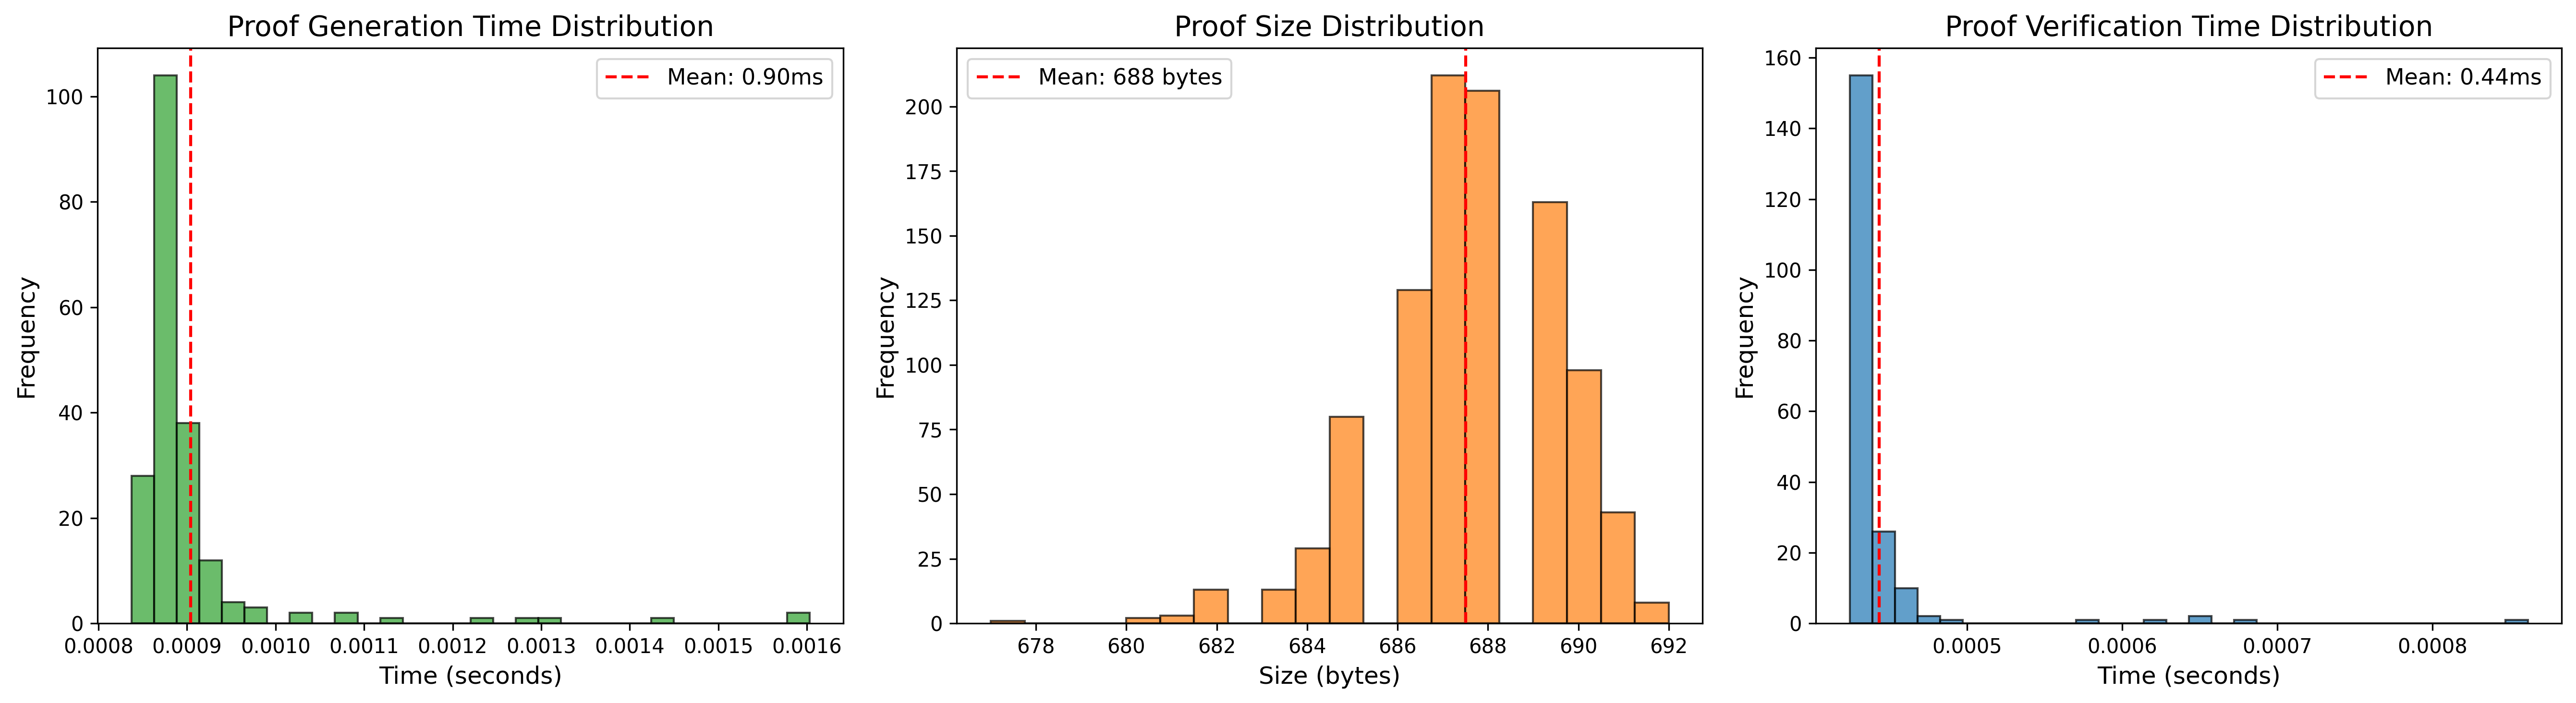
\includegraphics[width=\textwidth]{figures/zkp_overhead.png}
    \caption{Distribution of ZKP overhead. Left: proof generation times (${\sim}$1\,ms). Center: proof sizes (${\sim}$688 bytes). Right: verification times ($<$0.5\,ms).}
    \label{fig:zkp_overhead}
\end{figure}

\subsection{Blockchain Gas Cost Analysis}

Table~\ref{tab:blockchain} reports blockchain costs. At 30~gwei gas price and \$3,000 ETH, each verification costs ${\sim}$\$3.50 on mainnet. This can be reduced 50--100$\times$ via Layer-2 rollups (Optimism, Arbitrum), bringing costs below \$0.05. Batch amortization further reduces per-record overhead.

\begin{table}[t]
\centering
\caption{Blockchain Storage Costs}
\label{tab:blockchain}
\begin{tabular}{lc}
\toprule
\textbf{Metric} & \textbf{Value} \\
\midrule
Total transactions & 1,000 \\
Total blocks mined & 101 \\
Total gas consumed & 38,910,724 \\
Avg. gas per transaction & 38,911 \\
Avg. mining time per block & 15.03\,ms \\
Chain integrity verified & Yes \\
\bottomrule
\end{tabular}
\end{table}

\subsection{Pipeline Timing}

Total runtime was 16,679\,s (${\sim}$4.6\,h) on a T4 GPU. Training dominated at 9,476\,s (57\%), evaluation at 7,200\,s (43\%). The ZKP and blockchain layers added only 3.1\,s combined ($<$0.02\% of runtime), confirming negligible overhead.

% ============================================================
\section{Analysis and Discussion}
\label{sec:analysis}

\subsection{Security Analysis}

\textbf{Soundness.} The Schnorr-based protocol is $(2,3)$-special sound under the discrete logarithm assumption~\cite{schnorr1991efficient}. Forging a proof requires solving DLP on BN128, providing ${\sim}$128-bit security.

\textbf{Zero-Knowledge.} The protocol is honest-verifier zero-knowledge (HVZK). A simulator $\mathcal{S}$ produces indistinguishable transcripts by sampling $e', s_v', s_r' \xleftarrow{\$} \Z_q$ and computing $A' = g^{s_v'} \cdot h^{s_r'} \cdot C^{-e'} \bmod p$. The Fiat-Shamir heuristic achieves non-interactive ZK in the random oracle model~\cite{fiat1986prove}.

\textbf{Blockchain Immutability.} Altering block $B_i$ invalidates all subsequent blocks. Our experiments confirm 100\% detection of simulated tampering.

\subsection{Comparison with Existing Approaches}

Table~\ref{tab:comparison} compares ZK-KGVerify with related systems. ZK-KGVerify is the first to unify KGs, deep learning, ZKPs, and blockchain for privacy-preserving verifiable reasoning.

\begin{table}[t]
\centering
\caption{Comparison with Related Approaches}
\label{tab:comparison}
\begin{tabular}{lccccc}
\toprule
\textbf{System} & \textbf{KG} & \textbf{DL} & \textbf{ZKP} & \textbf{BC} & \textbf{Privacy} \\
\midrule
zkML~\cite{kang2022scaling} & \texttimes & \checkmark & \checkmark & \texttimes & \checkmark \\
zkCNN~\cite{liu2021zkcnn} & \texttimes & \checkmark & \checkmark & \texttimes & \checkmark \\
vCNN~\cite{lee2020vcnn} & \texttimes & \checkmark & \checkmark & \texttimes & Partial \\
BlockFL~\cite{kim2019blockchained} & \texttimes & \checkmark & \texttimes & \checkmark & Partial \\
DInEMMo~\cite{dinEmmo2021} & \texttimes & \checkmark & \texttimes & \checkmark & \texttimes \\
\textbf{ZK-KGVerify} & \checkmark & \checkmark & \checkmark & \checkmark & \checkmark \\
\bottomrule
\end{tabular}
\end{table}

\textbf{Overhead comparison.} Existing zkML approaches compile full forward passes into arithmetic circuits: zkCNN~\cite{liu2021zkcnn} reports 3--88\,s proof generation, EZKL~\cite{ezkl2023} requires 10--300\,s. ZK-KGVerify achieves $<$1\,ms by committing to model outputs rather than proving full inference---a deliberate trade-off suitable for applications where model integrity is established via auditing or certification.

\subsection{Limitations}

(1)~Our protocol proves predictions came from \emph{committed} parameters but does not verify the training process itself. (2)~The local blockchain simulation does not capture real-world network latency or fee dynamics. (3)~We evaluate on FB15k-237 with three models; extending to larger KGs and additional architectures is future work.

% ============================================================
\section{Conclusion}
\label{sec:conclusion}

We presented ZK-KGVerify, a framework bridging knowledge graph reasoning, zero-knowledge proofs, and blockchain for privacy-preserving verification of AI predictions. Our system generates cryptographic proofs for GNN-based KG predictions with ${\sim}$1\,ms overhead, achieving 100\% tamper detection with Ethereum-compatible gas costs. Future work includes verifiable training, Ethereum testnet deployment, federated KG construction with ZKP-verified contributions, and integration with production KG systems.

% ============================================================
\bibliographystyle{splncs04}
\bibliography{references}

\end{document}
